\chapter{Rund um den Kreis}

Autor: Marc Mittner

\section{Der Kreis}

Mathematisch korrekte Definition eines Kreises $ K $ in der Ebene $ E $:
\[ K \ = \ \lbrace X \ \in \ E \ \ , \ mit \ |\overline {MX}| \ = \ r \rbrace \]
Erl"auterung: K ist eine Menge, die alle Punkte $ X $ einer Ebene $ E $ enthält, für die gilt, dass die Länge der Strecke $ \overline {MX} $ gerade den Radius $ r $ ergibt.

\subsection{Mathematische Beschreibung}
Für die mathematische Beschreibung eines Kreises gibt es verschiedene Mög"-lich"-keiten. Hier soll vorerst nur die Darstellung mit kartesischen Koordinaten vorgestellt werden.

\subsection{Koordinatengleichung}

Die Koordinatengleichung eines Kreises im kartesischen Koordinatensystem:
\[ (x \ - \ x_M)^2 (y \ - \ y_M)^2 = r^2 \]
Der Mittelpunkt des Kreises ist dabei $ M = (x_M , y_M) $, der Radius des Kreises ist $ r $.

Diese Beziehung wird sofort durch den Satz des Pythagoras klar:

\begin{center}
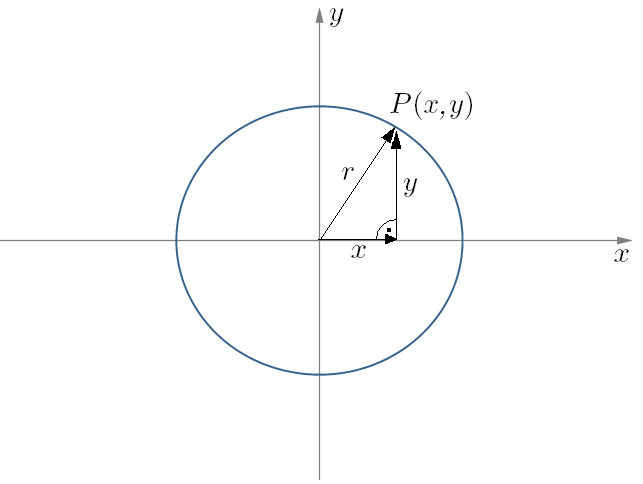
\includegraphics[width=0.6\textwidth]{img/Kreis.png}
\end{center}

$ x $ , $ y $ und $ r $ bilden ein rechtwinkliges Dreieck bilden. So ist mit dem Satz von Pythagoras sofort klar:
\[ x^2 \ + \ y^2 \ = \ r^2 \]
bei Mittelpunkt $ M \ = \ (0 , 0) $

Mit möglicher Verschiebung des Kreises in x- bzw. y-Richtung entsteht die Koordinatengleichung:
\[ (x \ - \ x_M)^2 (y \ - \ y_M)^2 = r^2 \]

\subsection{Funktionsgleichung}

Durch Umformen der Koordinatengleichung erhält man zwei Funktionsgleichungen zur Beschreibung des Kreises:
\[ y \ = \ y_M \ \pm \ \sqrt{ r^2 \ - \ (x \ - \ x_M)^2} \]

\subsection{Beispiele}

1)
Der Einheitskreis mit Radius $ r = 1 $ um den Ursprung $ M \ = \ (0 , 0) $:

\begin{center}
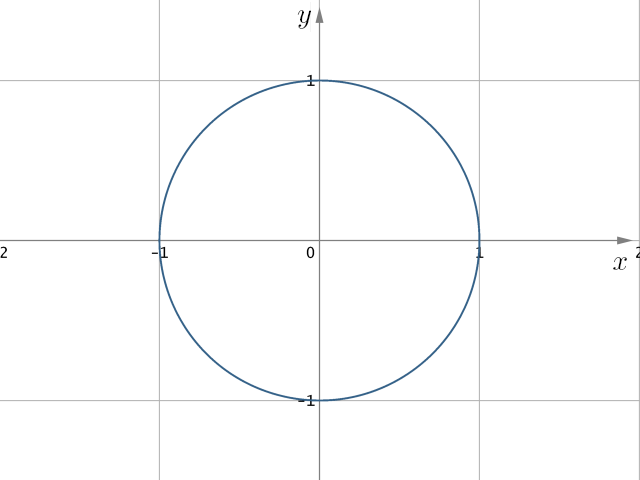
\includegraphics[width=0.6\textwidth]{img/Kreis1.png}
\end{center}

Koordinatengleichung:
\[x^2 \ + \ y^2 \ = \ 1 \]

\pagebreak
2)
Kreis mit Radius $ r \ = \ \sqrt 2 $ und Mittelpunkt $ M \ = \ (\sqrt 2 , \sqrt 2) $:
\nopagebreak
\begin{center}
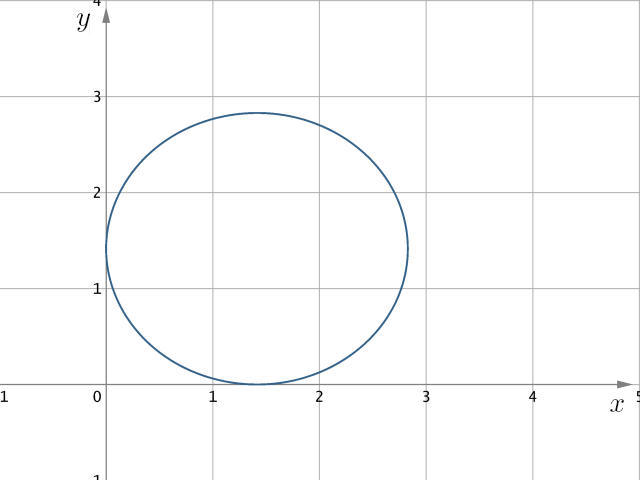
\includegraphics[width=0.6\textwidth]{img/Kreis2.png}
\end{center}

Koordinatengleichung:
\[(x \ - \ \sqrt 2)^2 \ + \ (y \ - \ \sqrt 2)^2 \ = \ 2 \]


3)
Oberer Halbkreis mit Radius $ r \ = \ 1.5 $ und Mittelpunkt $ M \ = \ (4 , 3) $

\begin{center}
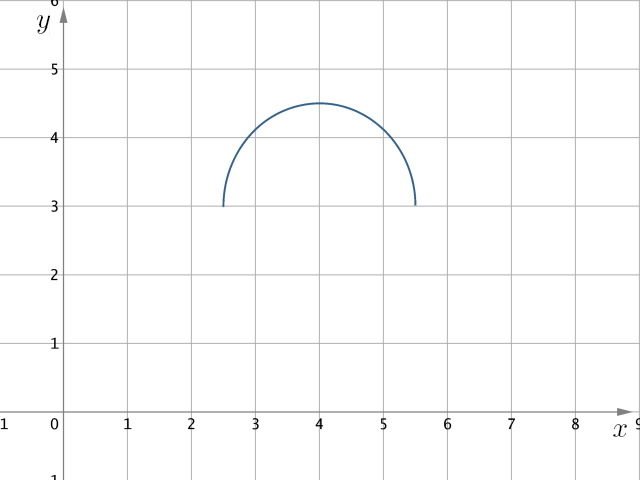
\includegraphics[width=0.6\textwidth]{img/Kreis3.png}
\end{center}
Funktionsgleichung: 
\[y = \ 3 \ + \ \sqrt{ 2.25 \ - \ (x \ - \ 4)^2} \]
